\documentclass[a4paper, 11pt]{article}

\setcounter{tocdepth}{3}
\setcounter{secnumdepth}{3}

\usepackage{comment} % enables the use of multi-line comments (\ifx \fi) 
\usepackage{lipsum} %This package just generates Lorem Ipsum filler text. 
\usepackage{fullpage} % changes the margin
\usepackage[utf8]{inputenc}
\usepackage{gensymb}
\usepackage{graphicx}
\usepackage{booktabs}% http://ctan.org/pkg/booktabs
\usepackage{makecell}
\usepackage{tabularx}
\usepackage[table]{xcolor}
\usepackage{array}
\usepackage{wrapfig}
\usepackage{subcaption}
\usepackage{csquotes}

\newcommand{\tabitem}{~~\llap{\textbullet}~~}
\newcommand{\shl}{~~\shortstack[l]}

\begin{document}
\title{Zusammenfassung Data Warehousing FS2018}
\author{Alex Neher}
\maketitle

\tableofcontents
\newpage

\graphicspath{{./Pictures/}}

\section{Die Notwendigkeit von Data Warehouses}
\subsection{Entscheidungsunterstützung (Buch S11)}
Data Warehouses sind keine neue Erfindung. Bereits in den 1960er Jahren wurden sogenannte \textbf{Managementsinformationssysteme} entwickelt. Diese MIS dienten dazu, Entscheidungsträgern alle benötigten Informationen zeitnah, fehlerfrei, flexibel, ergonomisch, effizient, effektiv und inspirativ zur Verfügung zu stellen.

Es gibt vier Arten der Entscheidungsunterstützung:

\begin{description}
	\item [Modellbasiert:] z.B. Lineare Optimierung - Ein Mathematischer Ansatz basierend auf einem Modell $\Longrightarrow$ Abbildung der Realität
	\item [Wissensbasiert: ] z.B. Expertensysteme - Ansätze von Künstlicher Intelligenz
	\item [Datenbasiert: ] Basierend auf grossen Datenmengen $\Longrightarrow$ Data-Warehouse, OLAP oder Data-Mining
	\item [KI: ] Basierend auf Vorschlägen von Systemen, die Entscheidungen auf Basis von Daten und/oder gelernten Inhalten ($\longrightarrow$ Machine Learning)
\end{description}

\subsubsection{Expertensystem}
Ein Expertensystem (XPS oder ES) ist ein Computerprogramm, das Menschen bei der Lösung von komplexen Problemen wie ein menschlicher Experte unterstützen kann, indem es Handlungsempfehlungen aus einer Wissensbasis ableitet.

\begin{figure}[htb]
	\centering
	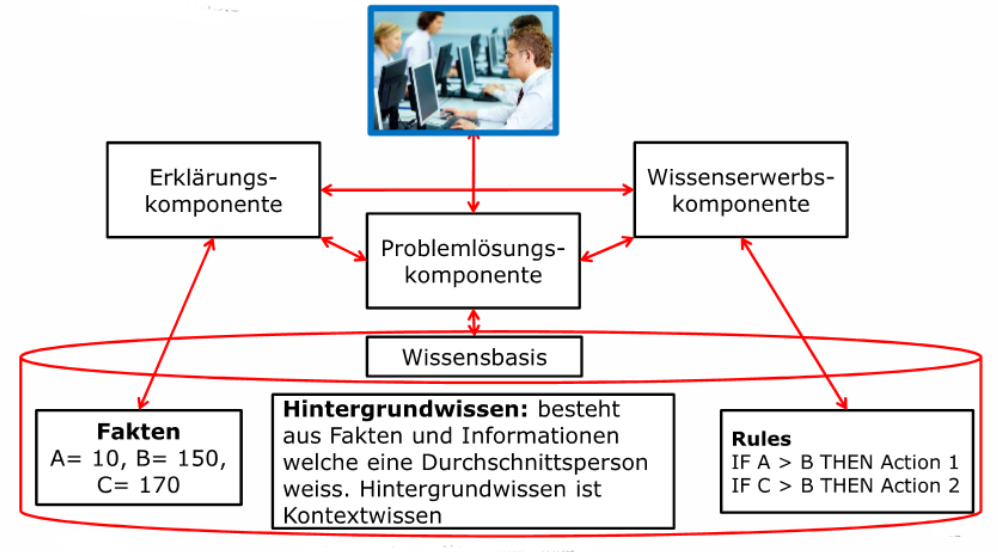
\includegraphics[keepaspectratio=true,height=18\baselineskip]{expertensystem.png}
	\caption{Beispiel eines Expertensystems}
	\label{fig:xps}
\end{figure}

\newpage

\subsection{Ungenügen der "gängigen" Datenhaltung (Buch S13)}

\begin{itemize}
	\item Verschiedene Datenformate
	\item Verschiedene Werkzeuge
	\item Heterogenität der Daten
		\subitem Technisch
			\subsubitem Mainframe
			\subsubitem DBMS
			\subsubitem Flatfile
		\subitem Logisch
			\subsubitem Schemata
			\subsubitem Formate
			\subsubitem Darstellungen
		\subitem Syntaktisch
			\subsubitem Datum
			\subsubitem Codierung
			\subsubitem Währung
		\subitem Qualitativ
			\subsubitem Fehlende Werte
			\subsubitem Falsche Werte
			\subsubitem Doppelte Werte
		\subitem Verfügbarkeit
			\subsubitem Permanent
			\subsubitem Periodisch
			\subsubitem Temporär
		\subitem Rechtlich
			\subsubitem Datenschutz
			\subsubitem Zugriffsverwaltung
			\subsubitem Archivierung
\end{itemize}

$\longrightarrow$ Neuer Ansatz einer Datenaufbereitung muss her: \textbf{Homogenisierung}

\subsection{Ungenügen der operativen Datenbanken für Entscheide (Buch S13)}

"Reguläre" Datenbanken im Geschäftsumfeld sind zu fest mit gesellschaftsrelevanten Lese- und Schreiboperationen beschäftigt. Bei solchen Datenbanken spricht man von OLTP-System (Online Transactional Processing). Diese Datenbanken sind aus Performance-Gründen ziemlich schlecht geeignet für eine analytische, vorausschauende Bewirtschaftung.

Ausserdem liegen Daten in OLTP-Datenbanken meist in der 3. Normalform vor. Während dies eine sehr vernetze und effiziente Art der Datenspeicherung ist, ist die 3. Normalform ein schlechtes Abbild des intuitiven Denkens eines Managers.

$\rightarrow$ Neuer Ansatz einer Datenbank muss her: \textbf{analytische Datenbanken}

\subsection{SQL-Abfragen für Management-Zwecke}
Zusätzlich zu den vorhin genannten Gründen, sind Manager des SQL meist nicht mächtig. Sie wollen lieben "Drag and Drop" Interfaces, um sich ihre Daten "zusammenzuklicken" wie z.b. Microsoft Access.

$\rightarrow$ Neuer Ansatz der Datenabfrage muss her: \textbf{OLAP}

\subsection{OLAP vs OLTP}

\begin{tabular}{|l|r|r|}
	\hline 
	Merkmal & OLTP System  & OLAP System  \\ 
	\hline 
	Ausrichtung auf & Programm, BWL Prozess & Mensch, Analyse\\ 
	\hline 
	Zeitliche Reichweite & Taktisch & Strategisch \\ 
	\hline 
	Entscheidungsstufe & Tief & Hoch \\ 
	\hline
	Zweck & Rationalisierung \& Automatisierung & Planung \& Entscheidung \\
	\hline
	Anwenderzahl &Hoch & Tief \\
	\hline
	Entscheidung & Deduktiv & Induktiv / Explorativ \\
	\hline
	Bewirtschaftung I & Ändernd & Befragend \\
	\hline
	Bewirtschaftung II & Auf Datensatzebene & Auf Aggregatsebene \\
	\hline
	Anwendungsmuster & Voraussehbar & Variierend \\
	\hline
	Befragungsmuster & Einfach & Komplex \\
	\hline
	Bearbeitung & Repetitiv & Ad hoc / unstrukturiert \\
	\hline
	Betriebliches Wissen & Verarbeitend & Generierend \\
	\hline
	Verteilungsgrad & Dezentral & Zentral \\
	\hline
	Performance-Bedarf & Durchgehend hoch & Variierend \\
	\hline
	Mehrbenutzersynchronisation & Hoch & Tief bis keine \\
	\hline
	Optimierung & Schneller Insert \& Delete & Schnelles Lesen \\
	\hline
	Transaktionsdurchsatz & Hoch & Tief \\
	\hline
	Transaktionsdauer & Kurte Mutationen weniger Tupel & Lange Abfragen vieler Tupel \\
	\hline
	Abfragen & Häufige, einfache Abfragen & Weniger häufige, komplexe Anfragen \\
	\hline
	Antwortzeiten & (Mili)sekunden & Sekunden, Minuten, Stunden \\
	\hline
	Endbenutzerwerkzeug-Hersteller & DB-Hersteller & Markt \\
	\hline
	Zeitbezug & Aktuell & Historisch \\ 
	\hline
	Zeitdimension & Zeitpunkt & Zeitraum \\
	\hline
	Beständigkeit & Dynamisch & Statisch \\
	\hline
	Granularität & Fein & Grob \\
	\hline
	Datenbestand & Vollständig & Lückenhaft \\
	\hline
	Redundanz & Normalisiert & Denormalisiert \\
	\hline
	Datenqualität / Aussagekraft & Tief & Hoch \\
	\hline
	Aufbereitung & Anwendungsneutral & Analyseorientiert \\
	\hline
	Aktualisierung & Laufend & Periodisch \\
	\hline
	Verarbeitungseinheit & Keon & Gross \\
	\hline
	Verteilungsgrad & Dezentral & Zentral \\
	\hline
	Datenquelle & Aktuelle Unternehmensdaten & Interne \& externe Daten \\
\end{tabular} 

\newpage

\section{Daten vs. Informationen vs. Wissen vs. Weisheit}

\begin{figure}[htb]
	\centering
	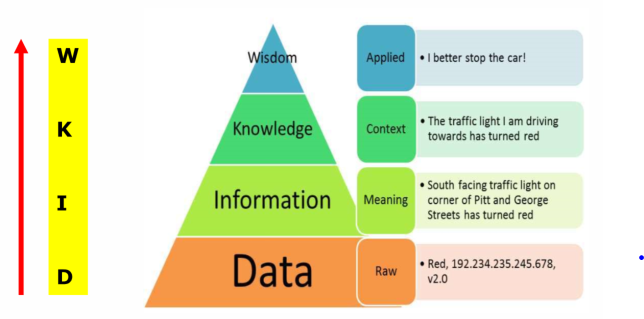
\includegraphics[keepaspectratio=true,height=18\baselineskip]{DIWW.PNG}
	\caption{DIKW-Pyramid}
	\label{fig:dikw}
\end{figure}

Bei Entscheidungsfindungen muss unterschieden werden zwischen

\begin{itemize}
	\item Daten
	\item Informationen
	\item Wissen
	\item Weisheit
\end{itemize}

\paragraph{Daten}
Daten sind das, was in Datenbanken oder Excel-Tabellen gespeichert wird. \textbf{Unstrukturierte Fakten} wie z.B die Zahlenreihenfolge 
\begin{center}
\textbf{	Rot, 192.234.235.245.678.v2.0}
\end{center}

\paragraph{Informationen}
Aus Daten alleine werden wir nicht schlau. Diese Daten müssen zuerst in einen \textbf{Zusammenhang} gebracht werden:

\begin{center}
\textbf{	Das südliche Rotlicht Pitt/George St. ist soeben rot geworden }
\end{center}

Nun können wir aus dieser, vorher völlig nutzlosen Zahlenreihe eine \textbf{Information} extrahieren. Nämlich dass sie Koordinaten sind und sich das "Rot" auf ein Lichtsignal bezieht..

Die Daten stellen zwar den eigentlichen Wert der Information dar (die Koordinaten und Rotlicht-Licht), sind aber ohne Zusammenhang völlig wertlos.

\paragraph{Wissen}
Aus Informationen \textbf{Wissen} zu machen ist nun, zumindest maschinell gesehen wesentlich schwerer. Wir Menschen generieren Wissen, indem wir Informationen geistig verarbeiten. Soll heissen, wir \textbf{interpretieren und ordnen} die gegebene Information.

Das heisst in diesem Fall, wir checken wo wir sind und in welche Richtung wir uns bewegen. Je nach dem ist das Wissen dann:

\begin{center}
\textbf{	Ich fahre in eine völlig andere Richtung, diese Information interessiert mich nicht.}
\end{center}

oder aber

\begin{center}
\textbf{	Das Rotlicht, auf welches ich zufahre, ist gerade rot geworden}
\end{center}

\paragraph{Weisheit}
Weisheit wird definiert als \textbf{Anwendung von Wissen auf eine Problemlösung}. Das heisst, das erworbene Wissen wird mit einer Portion Erfahrung und gesundem Menschenverstand gemixt. In unserem Fall, angenommen wir fahren auf das Rotlicht zu, sagt uns die Erfahrung, dass man bei einem roten Rotlicht stoppen soll und der gesunde Menschenverstand wirft noch ein, dass es entweder einen Unfall geben wird oder aber sicherlich eine Busse, sollte man erwischt werden. Das Ganze resultiert in:

\begin{center}
\textbf{	Ich sollte vermutlich nächstens einmal anhalten}
\end{center}

\vspace*{20px}

\begin{figure}[htb]
	\centering
	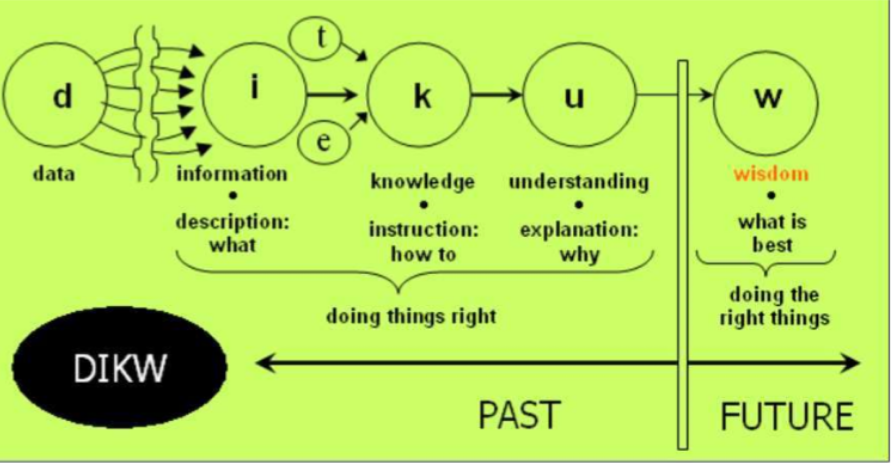
\includegraphics[keepaspectratio=true,height=15\baselineskip]{DIKW.PNG}
	\caption{Die Beziehung zwischen Daten - Informationen - Wissen - Weisheit}
	\label{fig:DIKW}
\end{figure}

Zusammengefasst kann man also sagen, Informationen sind das Verständnis von Zusammenhängen in Daten, oder auch \textbf{was die Daten bedeuten}. Wissen ist das Verständnis dieser Information (\textbf{was heisst das für mich?}) und Weisheit bestimmt, \textbf{was nun zu tun sei}. 
\newpage

%ToDo: Unterschied Daten, Information, Wissen, Weisheit??
\section{Das Data Warehouse}

\begin{wrapfigure}{R}{0.5\textwidth}
	\centering
	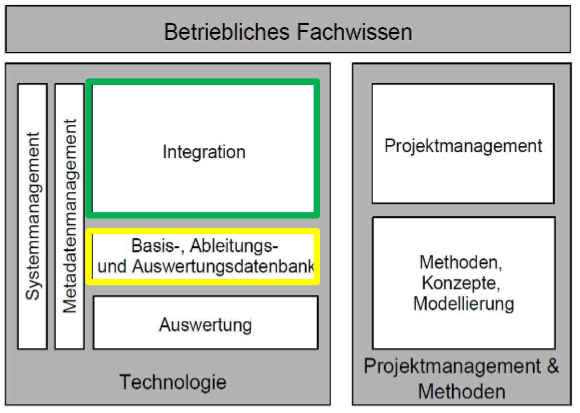
\includegraphics[keepaspectratio=true,height=10\baselineskip]{datawarehouse.PNG}
	\caption{Aufbau eines Datawarehouses}
	\label{fig:datawarehouse}
\end{wrapfigure}

In einer optimalen Welt würden Daten "perfekt" abgelegt werden, leicht zugänglich, platzsparend, sicher und für verschiedene Zwecke nützlich. Da wir aber leider nicht in einer optimalen Welt leben, ist dies nicht der Fall. (Buch S32)

Daten sind in der Praxis meist nicht optimal abgelegt. Daten existieren meist
\begin{itemize}
	\item in unterschiedlichen Formaten (Excel, Access, DB etc)
	\item in unterschiedlichen DB-Strukturen 
	\item in unterschiedlichen IT-Architekturen und -Systemen. Meist auch uralt Legacy-Systeme (Wie z.B. Cobol)
	\item zeit-aktuell und dynamisch
	\item zu detailliert und feingranular für wirksame Management-Abfragen
	\item in einem Format, das für Änderungstransaktionen optimiert wurde (z.B. 3. Normalform)
	\item mit begrenzten Zugriffsrechten (z.B. aus Security-Gründen)
	\item in einem schlecht verfügbaren Zustand (Legacy-System, proprietäres Format, Security-Gründe)
	\item in einem Format, welches komplexe SQL-Queries verlangt, um an Informationen oder Wissen zu gelangen.
\end{itemize}

$\rightarrow$ Lösung: \textbf{Data-Warehouse}

\subsection{Definition Data-Warehouse (Buch S 33)}
	
\blockquote[Oracle corp: Data warehousing Guide 11g (2007)]{A data warehouse is a relational database that is designed for query and analysis rather than for transaction processing. It usually contains historic data derived from transaction data, but can incude data from other sources. Data warehouses separate analysis workload from transactin workload and enable an organisation to consoldiate data from several sources.} 
 

\blockquote[IBM Corp: Enterprise Data Warehousing with DB2.9 - Redbook (2008)]{A data warehouse is a organisation's data with a corporate wide scope for use in decision support and informational applications.}
\vspace*{10px}

Zusammengefasst kann man also sagen, ein Data Warehouse ist eine Datenbank, welche nicht (ausschliesslich) zur Speicherung von Informationen genutzt wird, sondern hauptsächlich als Hilfsmittel bei Entscheidungen eingesetzt wird ($\rightarrow$ Experten-Systeme)



\subsection{Bestandteile eines Data-Warehouses (Buch S39)}

\begin{description}
	\item [SSRS: ] SQL Server Reporting Services
	\item [SSAS: ] SQL Server Analysis Services
	\item [SSIS: ] SQL Server Integration Services
\end{description}

\begin{figure}[htb]
	\centering
	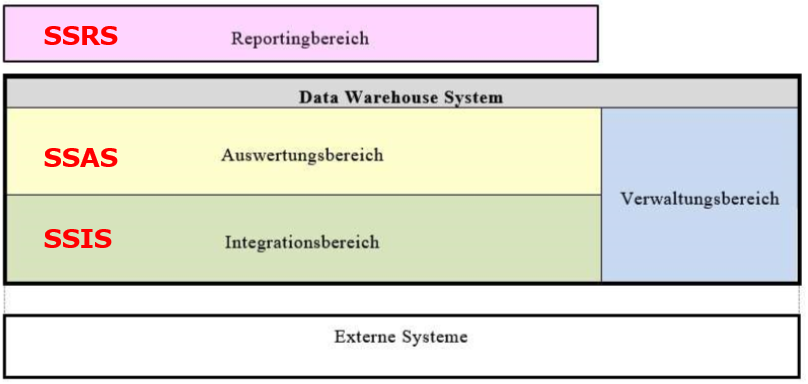
\includegraphics[keepaspectratio=true,height=18\baselineskip]{bestandteiledatawarehouse.PNG}
	\caption{Bestandteile eines Data-Warehouses}
	\label{fig:bstdw}
\end{figure}

\newpage

\subsection{Welche Datenbank für welche Tasks? (Buch S40f)}

\begin{figure}[htb]
	\centering
	\begin{subfigure}{0.45\textwidth}
		\centering
		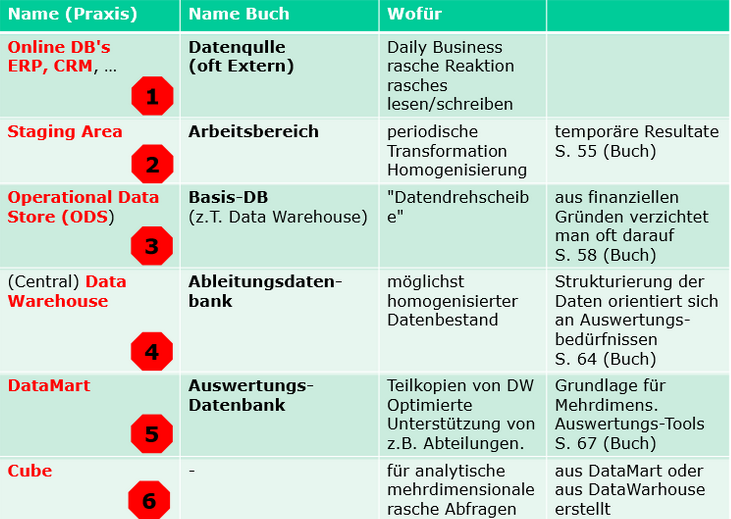
\includegraphics[width=\linewidth]{whichDB.PNG}
		\caption{Welche Datenbank für welche Tasks verwendet werden kann}
		\label{fig:whichDB}
	\end{subfigure}
	\begin{subfigure}{0.45\textwidth}
		\centering
		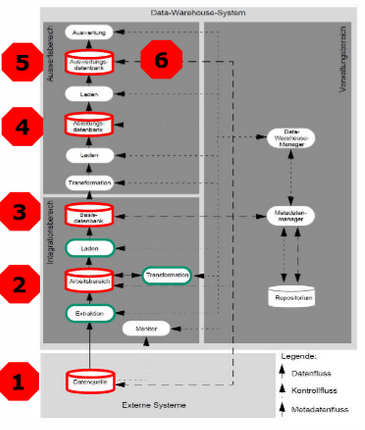
\includegraphics[width=\linewidth]{referenceArch.PNG}
		\caption{Referenzmodell nach Bauer \& Günzel}
		\label{fig:refArch}
	\end{subfigure}
\end{figure}

Verschiedene Datenbanken können (und sollten) für verschiedene Tasks verwendet werden.

\end{document}
